\documentclass{article}

\usepackage[utf8]{inputenc}
\usepackage[T1]{fontenc}
\usepackage{datetime}
\usepackage{graphicx}
\usepackage{float}
\usepackage{subcaption}

\usepackage{minted}
\usepackage[os=win]{menukeys}
\usepackage{tikz}

\usepackage[english]{babel}
\usepackage{geometry}

\usepackage{adjustbox}
\usepackage{multirow}
\usepackage{hyperref}
\usepackage{titlesec}

\geometry{
	a4paper,
	left=25mm,
	right=25mm,
	top=25mm,
	bottom=25mm,
}

\hypersetup{
	colorlinks=true,
	linkcolor=blue,
	urlcolor=blue,
}

\setcounter{secnumdepth}{4}
\renewcommand{\theparagraph}{\thesubsubsection.\alph{paragraph}}

\addto\captionsenglish{\renewcommand{\contentsname}{Daftar Isi}}
\addto\captionsenglish{\renewcommand{\tablename}{Tabel}}
\addto\captionsenglish{\renewcommand{\figurename}{Gambar}}

\def\mydate{\leavevmode\hbox{\the\year-\twodigits\month-\twodigits\day}}
\def\twodigits#1{\ifnum#1<10 0\fi\the#1}

% this custom commands below will not work if not run on GNU/Linux
\newcommand{\ShowOsVersion}{
	\immediate\write18{\unexpanded{foo=`uname -srom | tr '_' '-'` && echo -n "${foo}" > tmp.txt}}
	\unskip\unskip\input{tmp.txt}\unskip
	\immediate\write18{rm tmp.txt}
}
\newcommand{\ShowTexVersion}{
	\immediate\write18{\unexpanded{foo=`pdflatex -version | head -n1 | cut -d' ' -f1,2` && echo -n "${foo}" > tmp.txt}}
	\unskip\unskip\input{tmp.txt}\unskip
	\immediate\write18{rm tmp.txt}
}

\begin{document}
\begin{titlepage}
		\centering

		{
			\LARGE
			\bf
			Laporan Kegiatan Kalibrasi Simulator Telinga
		}

		\bigskip

		{
			\large
			\bf
			Tim Penelitian Audiometer Portable Elbicare
		}

		\vfill

		\begin{figure}[H]
			\centering
			
\includegraphics[width=250pt,angle=0]{images/elbicare-logo}
		\end{figure}

		\vfill

        \bigskip

        {
            \bf
            Achmadi ST MT dan M. Ammar Asyraf ST MT
        }
	\end{titlepage}

	\newpage

	\textbf{Tentang Dokumen}\\

	\noindent Dokumen ini ditulis menggunakan {\textbf{\ShowTexVersion}}pada sistem operasi {\textbf{\ShowOsVersion}}yang
	diupdate terakhir pada tanggal {\mydate} di jam \currenttime.\\

	Kode sumber dokumen ini dapat ditemukan di laman repositori proyek
	\url{https://github.com/VibrasticLab/pikoakustik2/tree/master/prototrial/dokumen/berita_acara/itb_july2023/test_calib}.

	\newpage

	\tableofcontents

	\newpage
	\section{Pendahuluan}

	Dokumen ini adalah rangkuman kegiatan kalibrasi perangkat simulator telinga menggunakan metode ruang dengung.

	\subsection{Tujuan Kegiatan}

	Tujuan utama kegiatan ini adalah mendapatkan rekaman derau yang dapat digunakan sebagai input acuan kalibrasi
	dari setiap unit simulator telinga dimana besar rekaman derau tersebut dibandingkan dengan Sound Level Meter terkalibrasi.

	\subsection{Waktu dan Tempat}

	Kegiatan ini dilakukan di Ruang Dengung dan Ruang Kedap Gedung Adhiwijogo di Institut Teknologi Bandung pada tanggal 7 Juli 2023.

	\subsection{Alat dan Perlengkapan}

	Alat yang digunakan meliputi:

	\begin{itemize}
		\item Speaker merek Yamaha dengan Amplifier board portabel.

		\begin{figure}[H]
			\centering
			\begin{subfigure}[]{.45\textwidth}
				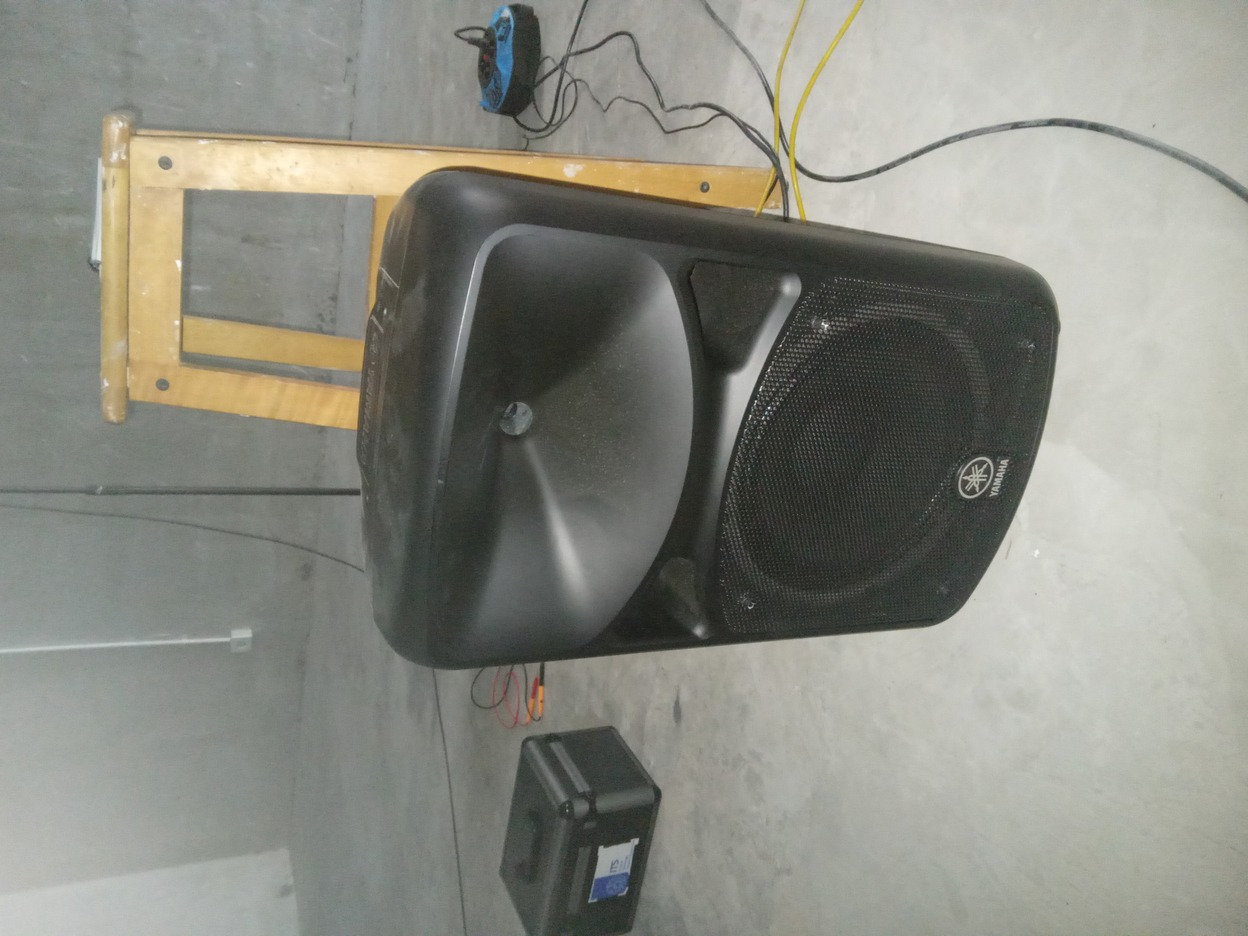
\includegraphics[width=\textwidth,angle=-90]{images/tools_speaker}
				\caption{Speaker}
			\end{subfigure}
			\begin{subfigure}[]{.45\textwidth}
				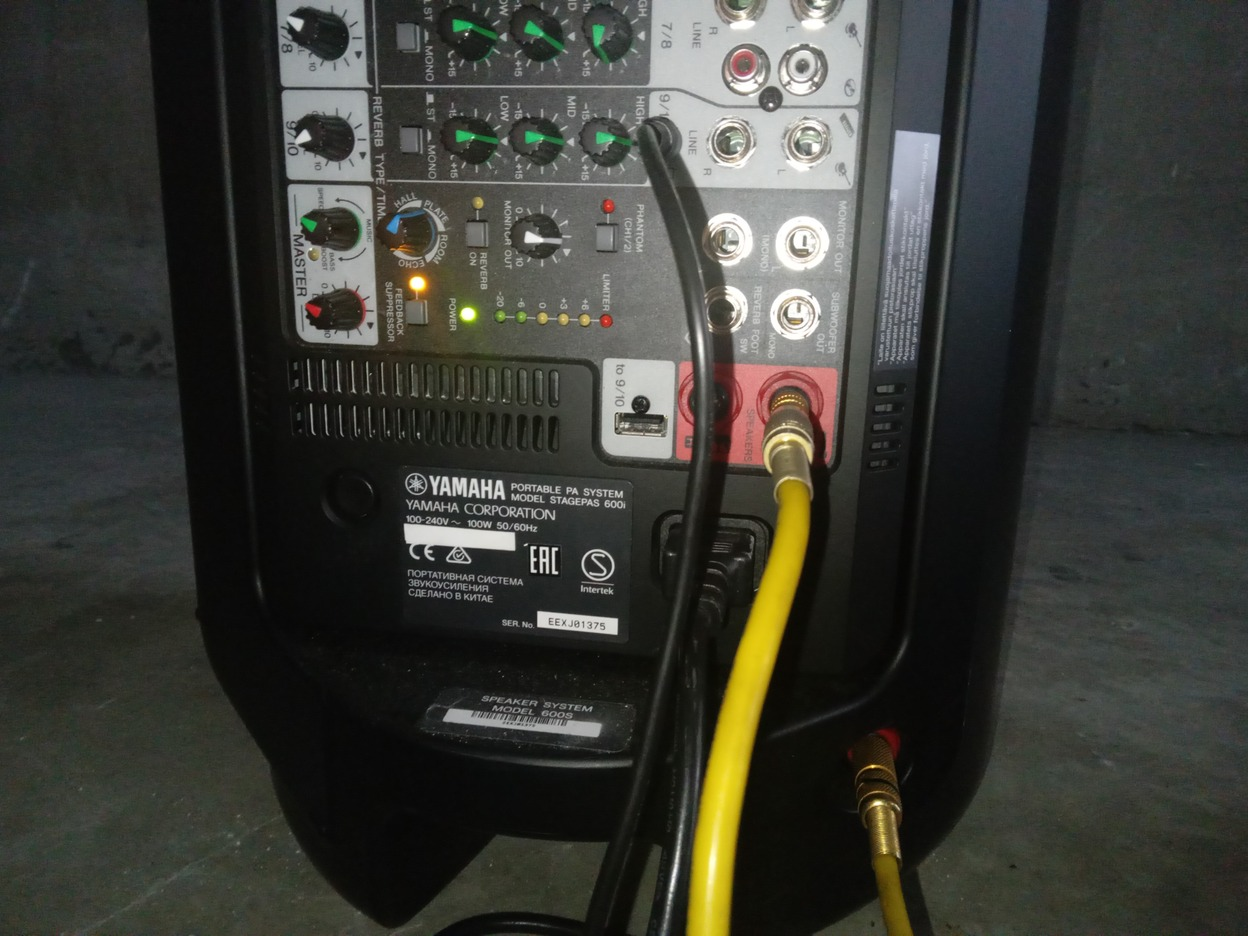
\includegraphics[width=\textwidth]{images/tools_amplifier}
				\caption{Amplifier}
			\end{subfigure}
			\caption{Perangkat Speaker}
		\end{figure}

		\item Sound Level Meter Merek Rion yang telah terkalibrasi.

		\begin{figure}[H]
			\centering
			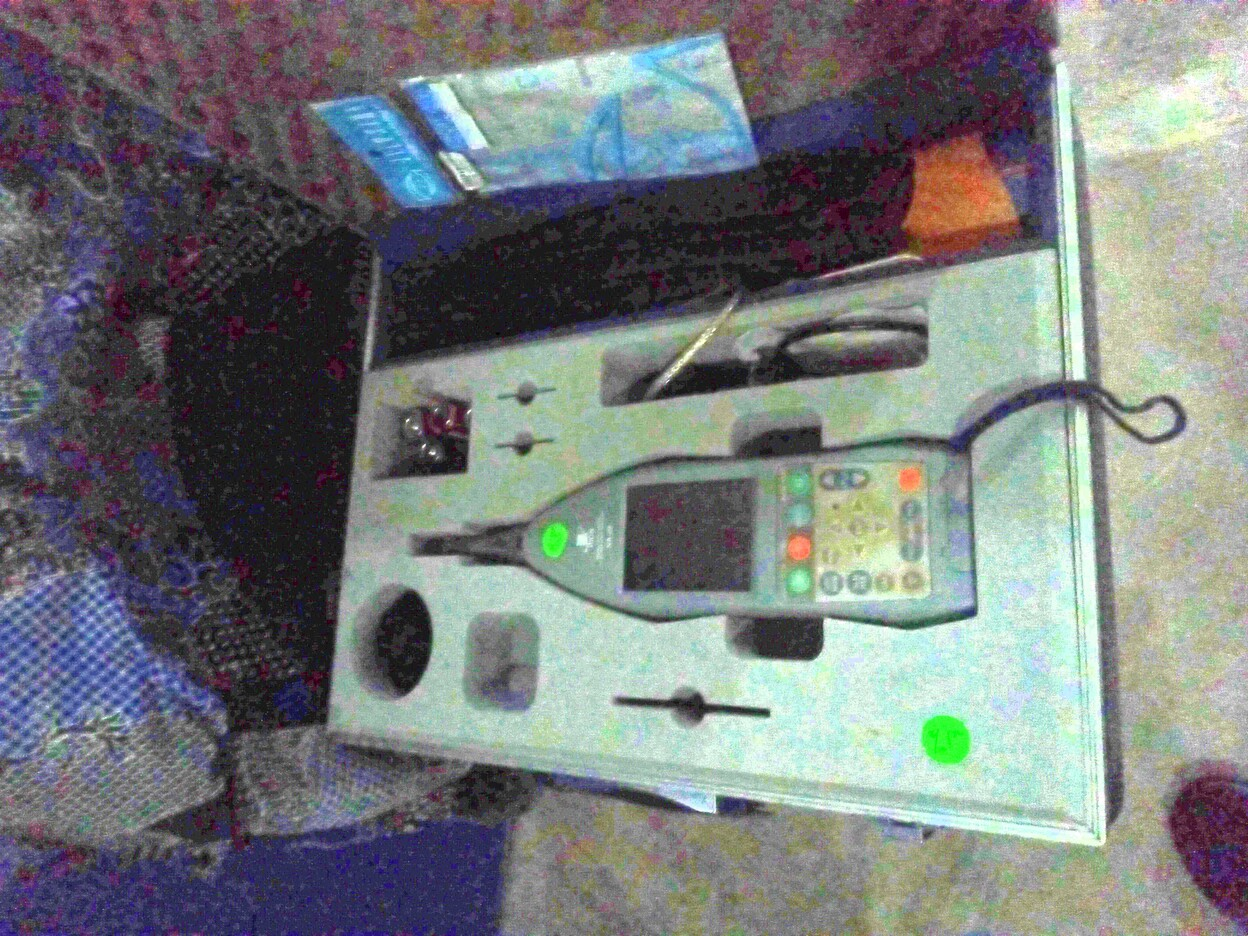
\includegraphics[width=180pt,angle=0]{images/tools_slm_box}
			\caption{SLM RION}
		\end{figure}

	\end{itemize}

	\subsection{Persiapan Kegiatan}

	\newpage
	\section{Kegiatan Kalibrasi}

	\subsection{Unit EARS}

	\subsubsection{Setup}

	\subsubsection{Recording}

	\subsubsection{Testing}

	\subsection{Unit 3DIO}

	\subsubsection{Setup}

	\subsubsection{Recording}

	\subsubsection{Testing}

	\subsection{Tes Ruang Kedap}

\end{document}
